\newcommand{\itmref}[2]{\hyperref[#2]{#1 Variable~\ref*{#2}}}

\section{Methodology}\label{sec:methodology}
The goal of this research was to empirically analyze each identificaton method, and determine which method most
accurately maps a subset of stars from the catalog to image under the presence of noise.
The general flow of experiments is listed below:
\begin{enumerate}
    \item \textit{Generate} (\autoref{subsec:benchmarkDataGeneration}) an image of stars.
    \item Apply noise to the image.
    \item Give the image to the identification method.
    \item Run the method to a certain step.
    \item Record the output.
    \item Repeat for another image.
\end{enumerate}

The research goal is directed toward star tracker development, who's input is often very noisy.
Before a raw image can be used in a star identification algorithm it must first go through some process to filter out
extraneous light.
From here, centroid coordinates of an image (i.e.\ stars) are determined in 2D using a \textit{center-of-mass} approach.
The coordinates are then projected from 2D to the 3D image frame, and then run through the star identification
algorithm.

There are a number of places where error can be introduced here.
What if the filtering removes a star?
What if centroid coordinates are inaccurately determined?
What if the 2D to 3D transformation is inaccurate as well?

In order to precisely quantity star identification error, a process must be created to produce an accurate
representation of the 3D image frame.
The exact stars in the image must be known, the date of the image, the field-of-view of the camera, what type of
error exists in the image, \ldots.
As much of the image is supposed to be known, while only varying the star identification algorithm itself.

Unfortunately, obtaining actual images with characterized error is incredibly difficult and not the focus of this
project.
The solution presented here is to remove the reliance on the camera to capture images, and instead
\textit{generate} the images from the catalog used to build the features from.
This allows for controllable hardware (field-of-view, camera direction are now just parameters) and for controllable
error, as the entire image to 3D image frame are cut out.

These images are generated using the Hipparcos Input Catalogue v2, an astronomical catalog of recorded stars and their
position relative to Earth.
Once the images were generated, three experiments were performed: one for feature uniqueness, one for reduction
effectiveness, and one for identification performance and accuracy.

All trials were performed on an Intel i7-7700 CPU, 3.60GHz with 16 GB RAM\@.
Each algorithm was implemented in C++17, and compiled without optimization (at \texttt{-O0}).
The exact implementation is available at the following link: \newline
\url{https://github.com/glennga/hoku}.

\subsection{Benchmark Data Generation}\label{subsec:benchmarkDataGeneration}
Benchmark images were generated with the process below:
\begin{enumerate}
    \item Choose a field-of-view, \textit{true attitude}, and an image center.
    \item Select all stars from the catalog that are within the field-of-view of the image center.
    \item Rotate all of these stars from the \textit{catalog frame} to the image frame using the true attitude.
    \item Give the rotated stars, the field-of-view, and the rotated image center to the star identification method.
\end{enumerate}

\begin{subequations}
    \label{eq:catalogToCartesian}
    The catalog here does not refer to the raw Hipparcos Input Catalogue using spherical coordinates, rather a
    modified catalog whose entries exist in a 3D cartesian frame.
    Depicted below is the conversion to ($x, y, z$) points, assuming $\alpha$ and $\delta$ are in radians:
    \begin{align}
        x &= d \times cos(\delta) cos(\alpha) \\
        y &= d \times cos(\delta) sin(\alpha) \\
        z &= d \times sin(\delta)
    \end{align}
\end{subequations}

$d$ in~\autoref{eq:catalogToCartesian} represents the distance from the Earth (an observer) to the star.
For this set of experiments, $d = 1$ to normalize each vector and work entirely on the celestial sphere.
Also stored with each star's ($x, y, z$) position are the star's apparent magnitude (brightness) $m$ and catalog
identifier $\ell$.
\textit{For simplicity, the \underline{catalog} refers to the set of stars in this Cartesian frame.}

As mentioned before, all catalog stars exist in an inertial frame known as the \textit{catalog frame}.
To generate clean benchmark images, three items must be specified:
\begin{itemize}
    \item An image center in the catalog frame $c_r$.
    \item The field-of-view of the camera $f$.
    \item True attitude to take stars in the catalog frame to the image frame $q_{rb}$.
\end{itemize}

Note that the goal of attitude determination is to find this true attitude $q_{rb}$.

\begin{figure}
    \centering{
    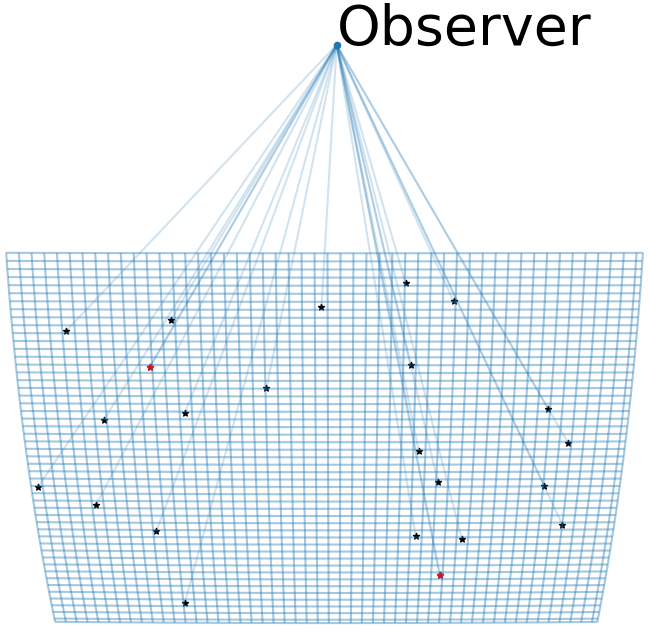
\includegraphics[scale=0.4]{images/benchmark.png}
    \caption{
    Visualization of an image presented to a star identification procedure.
    Stars are represented as vectors whose origin is the observer (i.e.\ Earth), and whose endpoint lies on a section
    of the celestial sphere.
    } \label{figure:benchmarkImageExample}
    }
\end{figure}

All stars $S_r$ from the catalog are selected such that no star exists more than $f$ away from $c_r$.
$S_r$ and $c_r$ are then rotated by $q_{rb}$ to construct the image stars: $S_b$ and $c_b$.
$S_b$ is then stripped of their catalog identifiers, as it is the job of the identification method to guess these.
The resulting image is presented in~\autoref{figure:benchmarkImageExample}.
What is presented to each identification method are the stars in the image $S_b$, the center of the image $c_b$, and
the field-of-view $f$.

% Citation: Pyramid method, pg14
Noise is assumed to exist in two forms here: misrepresentations of the centroid (i.e.\ centroiding error) and as
falsely identified sources of light in the image.
Centroiding error is applied to $S_b$ by slightly rotating a star $s$ in a random direction, whose severity is
determined by a Gaussian distribution $N(0, \sigma^2)$.
For this set of experiments, $\sigma = 50\mu rad$.
False stars were added to $S_b$ by generating a random vector $s$ within $f$ of $c_b$.

\subsection{Which set of features best distinguish a set of stars?}\label{subsec:featureUniquenessMethods}
This experiment helps determine which identification method has the best querying process for catalog candidates $R$.
This is the first filter step, reducing the entire catalog to a subset of combinations.
If the correct stars do not exist here (filter produces false negatives), then the following steps will not be able to
correctly determine a map.
On the other hand if not enough of the catalog is filtered, there is a greater chance of error occurring at later steps.

Differences in catalog querying are specified in each paper (K-Vector, KD Trees, \ldots), but in this set of
experiments all catalog querying uses a B-Tree index.
The only unique portion of each query that remains are what features each method uses to search the catalog.
The relational algebra then becomes:
\begin{equation}
    \Pi_{r_1, r_2, \ldots, r_k} (\sigma_{(c_f < q_f + 3\epsilon) \bigwedge (c_f > q_f - 3\epsilon)}(C))
\end{equation}

Here, $k$ refers to the number of stars used in the query (e.g. the Angle method uses $k = 2$ stars), $c_f$ refers to
the catalog feature amongst $r_1, r_2, \ldots, r_k$, $q_f$ refers to the image feature amongst a body set $b$,
$\epsilon$ refers to the deviation of noise, and $C$ refers to the catalog.

Toloei's Composite Pyramid uses the same features as Cole and Crassidus's Planar Triangles method, so only five
features were tested:
\begin{itemize}
    \item Angular separation $\theta^{ij}$ between two stars.
    \item Angular separations $\theta^{ic}, \theta^{jc}$ and interior angle $\phi$ between three stars.
    \item Planar area $a^{ijk}$ and moment $\imath^{ijk}$ between three stars.
    \item Spherical area $a^{ijk}$ and moment $\imath^{ijk}$ between three stars.
    \item Angular separations $\theta^{ij}, \theta^{ik}, \theta^{jk}$ between three stars.
\end{itemize}

The feature uniqueness of each identification method were analyzed in terms of three variables:
\begin{enumerate}
    \item \label{itm:featureDist} Feature distribution across all possible combinations of stars in the catalog.
    \item \label{itm:hitCountFeature} \textit{Query hits} from single catalog candidate searches.
    \item $|R|$ from single catalog candidate searches.
\end{enumerate}

TODO: Talk about the selectivity of each statement here?
TODO: Still need to determine how distribution is going to be quantitatively analyzed.

Query hit count here refers to finding a specific set of stars (the ones used to query for $R$) in the candidates.
Single catalog candidate searches refer to feeding an image to each identification method and running it to produce
an $R$ set.
Referencing~\autoref{figure:genericIdentificationMethodFlowchart}, this consists of performing the \textit{Get Camera
Image} step and executing the identification method past the \textit{Search Catalog} step to the first decision
block.
$R$ would then be analyzed for hits.

A more even distribution of features, a higher query hit count, and a smaller $|R|$ suggest a better chance of uniquely
identifying candidates.

\subsection{What is the best process for reducing catalog candidates?}\label{subsec:candidateReductionMethods}
This experiment helps determine which identification method has the best querying + candidate reduction process.
If a reduction process is too restrictive, then a single match in $R$ will never be found.
If a reduction process is not restrictive enough, then the following steps will rarely determine a correct map.

Referencing~\autoref{figure:genericIdentificationMethodFlowchart}, the experiment starts at the \textit{Get Camera
Image} step and executes the identification method to past the \textit{Confident in $r$?} decision block to produce a
single match $r$ for some $b$.

To characterize the reduction portion, the reduction process must be isolated.
Only results that pass the first filter (the previous experiment) step will be counted, to avoid characterizing the
query \textit{and} the reduction steps.
The number of correctly reduced $R$ sets with a query experiment hit was recorded against the number of incorrectly
reduced $R$ sets with a query experiment hit.

For a majority of these methods, a reduction process is a matter of repeating the query steps until $|R|=1$ holds true.
For the triangle methods however, their reduction process is the \Call{Pivot}{} method.
The experiment reduces down to $|R|=1$ reduction vs. \Call{Pivot}{} reduction, coupled with each individual method's
query steps.

To start, complete images were generated containing $S_b$, $c_b$, and $f$.
Each identification method was run until a singular set $r$ in $R$ is found.
If all $r$ exists in the original set $S_r$ used to generate the image, then this was counted as a
\textit{reduction hit}.

A higher reduction hit count suggests a more accurate feature set and reduction process.

\subsection{Which method most accurately determines a map?}\label{subsec:identificationMethods}
This experiment helps determine which identification method produces the most accurate catalog to image maps, running
the entire process from end to end.
An accurate map will reduce an attitude determination problem to Wahba's problem, which can be solved.

Referencing~\autoref{figure:genericIdentificationMethodFlowchart} again, this experiment runs the identification
method end to end.
To characteize the identification portion, the mapping process must be isolated.
Only results that pass the first and second filter (the previous experiment) steps will be counted, to avoid
characterizing the entire identification method.
The number of correct maps with the correctly reduced sets was recorded against the total number of incorrect maps
with correctly reduced sets.

The end to end trials were analyzed using two variables:
\begin{enumerate}
    \item \label{itm:correctReducedCandidates} Number of correctly reduced candidate sets $R \rightarrow r$.
    \item Number of correct maps in~\itmref{Map Experiment}{itm:correctReducedCandidates}.
\end{enumerate}

To start, complete images were generated containing $S_b$, $c_b$, and $f$.
Each identification method was run from start to finish, producing a map $a$ (or not one at all).
If the map references the correct stars in $S_b$ (i.e.\ the reduction experiment), this is recorded as a
\textit{reduction hit}.
If the map references the correct stars and the map $a$ is accurate, this is recorded as a \textit{map hit}.

A larger map to reduction hit ratio suggests a more accurate map determination process.